% !TeX root = RJwrapper.tex
\title{Asymptotic benchmarking using the \pkg{atime} package}
\author{Doris Amoakohene, Anirban Chetia, Toby Hocking}

\maketitle

\abstract{}
Time and memory efficiency are important features of statistical software.
When several different implementations of a given algorithm are available, benchmarking can be used to determine which is most efficient for a given task.
Typical benchmarking tools provide support for comparing time/memory usage of different computations for a data set of a given size $N$.
In this paper, we present the \pkg{atime} package, which provides asymptotic benchmarking, meaning that time and memory (as well as other quantities) can be easily measured for a sequence of increasing data sizes. 
Asymptotic measurement allows estimation of complexity classes (big-O notation), and provides a robust new method for testing the performance of R packages.
This paper provides a detailed comparison of \pkg{atime} with similar packages, and a discussion of how \pkg{atime} has been used to improve efficiency in base R and \pkg{data.table}. 

\section{Introduction}

Software efficiency, particularly in terms of time and memory usage, is a critical factor in computational research and analysis. As the scale and complexity of data continue to grow, the need for optimized code and algorithms becomes essential. 
Therefore, benchmarking package performance is important, as it allows us to identify the best package and function for specific tasks based on time and memory efficiency. 

For example, the task of writing a large CSV file can be accomplished by various functions, each with different performance characteristics. 
In R, the \texttt{base::write.csv} function is a standard approach for writing CSV files \citep{baseR}.
The R package \pkg{data.table} offers a highly efficient \texttt{fwrite} function, optimized for speed and large datasets \citep{data.table}. 
The \texttt{readr::write\_csv} from the \pkg{readr} package is another CSV writing function \citep{readr}.
In Python, there are other functions for CSV writing, such as \texttt{pandas.DataFrame.to\_csv()} and \texttt{dask.dataframe.to\_csv()}  \citep{pandas, dask}.
To compare the performance of these functions, common practice is to use tools like \pkg{microbenchmark} \citep{microbenchmark} or \code{bench::mark} \citep{bench}, which runs each function on a dataset of fixed size $N$, and reports metrics such as execution time and memory usage.  

However, running benchmarks using a single data size $N$ can be misleading, because the chosen data size $N$ may not be representative of typical use cases.
Since most real-world use cases involve large data sizes $N$, we propose an asymptotic benchmarking system, where the same code is measured across varying data sizes. 
For example, instead of benchmarking functions only for writing a CSV file with $N = 100$ rows, we can also run them with $N = 1000$ rows, and so on. 
By doing this, we can not only observe how fast an algorithm is at a specific input size, but also how its performance evolves as the data size grows. 
This type of analysis makes it possible to estimate asymptotic complexity classes (big-O notation), which tells us how the time or memory usage grows as a function of data size $N$ (linearly, exponentially, etc).


In this article, we focus on two kinds of analyses: comparative benchmarking, and performance testing, which we define below.
\paragraph{Comparative benchmarking.}
We use the term ``comparative benchmarking'' for efforts that aim to compare performance (typically time and memory usage) of different functions that do the same computation (for example, different functions for writing CSV files).
By comparing the performance of these different functions, the aim is to help users make informed choices about what software is most efficient for a particular data manipulation or analysis operation.
\paragraph{Performance testing.}
We use the term ``performance testing'' to refer to testing to ensure that the software stays efficient when the code is updated (for example, making a change to the source code of a function for writing CSV files). 
Note that performance testing is a special case of comparative benchmarking, where the different functions to compare are different versions (before and after updating the function's code). 
The goal is for package developers to be able to see if their code updates affect performance (time or memory usage).
We use the term ``continuous performance testing'' for the automated and ongoing assessment of performance (time and memory usage), as part of the development workflow. 
Another term is ``continuous benchmarking,'' which is a synonym used by Bencher, a web application that provides a graphical user interface for visualizing historical results \citep{bencher}.
We propose a system based on GitHub Actions, where performance testing is run for each commit of a Pull Request, and results can be used to avoid performance regressions, before merging each Pull Request.

In this paper, we present a detailed comparison of \pkg{atime} with existing benchmarking tools, demonstrating how it can be used to improve performance in R packages like \pkg{data.table}.


\section{Related work}
In this section, we summarize several related software tools for comparative benchmarking and performance testing
(Table~\ref{tab:comparison}).

\subsection{Comparative Benchmarking}

Several software packages provide comparative benchmarking functionalities.
Base R's \code{system.time()} provides a quick way to measure the execution time of one piece of R code, for one data size \citep{baseR}. 
\pkg{rbenchmark} wraps \code{system.time} to evaluate multiple expressions in a specified environment \citep{rbenchmark}.
\pkg{microbenchmark} provides nanosecond-precision timing of multiple R expressions \citep{microbenchmark}, with controls such as randomization of execution order (but without memory measurement).
\code{bench::mark()} measures time and memory usage of several pieces of code \citep{bench}, for a single data size (and this is what our proposed \pkg{atime} package uses internally).
While \code{bench::press()} could be used to measure time/memory usage for different data sizes, the proposed \pkg{atime} package provides a similar method with two advantages.
First, \pkg{atime} offers a faster approach, which stops measurement if the median time exceeds a certain threshold. 
Second, sometimes it is desirable to save results of each expression (for example, to check if the results are consistent).
In that case, \code{bench::mark(check=TRUE)} can be used to automatically stop with an error, if any pair of results is not equal.
In contrast, the proposed \code{atime(result=TRUE)} saves results but does not stop automatically, so the user can implement their own checks, which is more flexible.

\subsection{Performance Testing}

There are several other software packages which provide functionality for performance testing (Table~\ref{tab:comparison}).
\pkg{airspeed velocity} is a Python library for performance testing \citep{airspeed_velocity}, which is used by the numpy and pandas project \citep{numpy,pandas}. 
Different tests are run for a given code version and data size, and then results are saved to disk, creating a historical result.
Performance is tested by comparing the results for the current code with the historical results.
This approach can be useful if the data size is definitely relevant, and the results are always computed on the same computer.
However, the usefulness of this approach can be limited, because of two factors. 
First, different data sizes are relevant for testing on different computers, so some of the benchmarks could be irrelevant on a given computer (if the size is too small). 
Second, each version of the code to test is typically run on a different job under continuous integration services such as GitHub Actions. 
With such a setup, it is rarely possible to guarantee access the same computer, which means that important variations in code versions can be mistaken for insignificant variations over multiple different servers.
This type of performance testing system therefore results in a high level of false positives (system says there is a performance regression, but there actually was just noise due to using different servers).
Other similar tools include
\pkg{conbench}~\citep{conbench}, 
and \pkg{bencher}~\citep{bencher}.

\citet{pytest_benchmark} proposed the \pkg{pytest-benchmark} which integrates \pkg{airspeed velocity} benchmarking into \pkg{pytest}, which is a framework for unit testing.
Typically, unit tests are defined for small data sets, which are not relevant to performance testing, so the usefulness of this approach is limited.

In contrast, we propose a performance testing method which overcomes the drawbacks of the previous approaches.
To overcome the first drawback (fixed data size), we propose to define each test as a piece of code that is a function of the data size, \code{N}. 
The code is run for increasing data sizes, until the median time taken is greater than some threshold (default 0.01 seconds), which can be used to ensure that the largest data sizes are relevant for performance testing.
To overcome the second drawback (historical runs of different versions on different servers), we propose to keep a historical database of known fast/slow versions.
Instead of running each test using only the current version of the code (HEAD in git terms), we additionally propose to run each test using the known fast/slow versions, along with any other versions that are relevant in the context of a pull request (CRAN, base, merge-base).
The advantage is that this approach eliminates most false positives, since all measurements are computed on a single computer, in the same R session.
The drawback is that this approach requires more computation time during each run to install and test several versions of the code (instead of just the most recent version). 
Our proposed method is similar to the ``relative continuous benchmarking'' concept on \pkg{bencher} \citep{bencher}, which is limited to testing a single data size, using two code versions (main and feature branch); this concept is also implemented in 
\pkg{touchstone}~\citep{touchstone}.

\begin{table}[t]
\centering
\caption{Comparison of software for Comparative Benchmarking (Comp. Bench.) and Performance Testing (Perf. Test.).}
\label{tab:comparison}
\begin{tabular}{|m{3cm}|m{4em}|m{4em}|m{8em}|m{3em}|m{3em}|}
\hline
\pkg{}                & \pkg{Language} & \pkg{Users} & \pkg{Result Display} & \pkg{Comp. Bench.} & \pkg{Perf. Test.} \\ \hline
\pkg{atime} (proposed) & R                & \pkg{data.table}     & PR comments                            & yes                              & yes                         \\ \hline
\pkg{bench}            & R                &               - & -                                      & yes                              & -                           \\ \hline
\pkg{microbenchmark}   & R                &    -           & -                                      & yes                             & -                           \\ \hline
\code{system.time}      & R                &              - & -                                      & yes                              & -                           \\ \hline
\pkg{rbenchmark}       & R                &               - & -                                      & yes                              & -                           \\ \hline
\pkg{airspeed velocity} & Python          & \pkg{numpy}, \pkg{pandas}          & web page                               & -                                & yes                         \\ \hline
\pkg{conbench}         & any              & \pkg{arrow}          & web page                               & -                                & yes                         \\ \hline
\pkg{touchstone}       & R                &               - & PR comments                            & -                                & yes                         \\ \hline
% \pkg{pytest-benchmark}  & Python          &               - & web page                               & -                                & yes                         \\ \hline
\end{tabular}
\end{table}

\section{Example of comparative benchmarking using \pkg{atime}}
In this section, we demonstrate how \pkg{atime} can be used for comparative benchmarking.
We use the example of benchmarking R code for text processing using regular expressions (regex), using either \code{PCRE} or \code{TRE}, which are two C libraries that provide similar regex functionality.
\citet{PCRE} introduced \code{PCRE} which stands for Perl-Compatible Regular Expressions, and \citet{TRE} proposed \code{TRE} which is an approximate regular expression matching library.
With base R functions like \code{regexpr()}, \code{PCRE} is used when \code{perl=TRUE} and \code{TRE} is used when \code{perl=FALSE}.
We can compare the performance of these two libraries using \pkg{atime}, and the first step is to define a vector of data sizes, as in the code below.



\begin{Schunk}
\begin{Sinput}
> (subject.size.vec <- unique(as.integer(10^seq(0, 3, l=100))))
\end{Sinput}
\begin{Soutput}
 [1]    1    2    3    4    5    6    7    8    9   10   11   12   13   14   15
[16]   16   17   18   20   21   23   24   26   28   30   32   35   37   40   43
[31]   46   49   53   57   61   65   70   75   81   86   93  100  107  114  123
[46]  132  141  151  162  174  187  200  215  231  247  265  284  305  327  351
[61]  376  403  432  464  497  533  572  613  657  705  756  811  869  932 1000
\end{Soutput}
\end{Schunk}

In the code above, we created a sequence of integer values that will be used to define different data sizes to test with each library.
Using a grid of values on the log scale (\verb|10^seq|), is recommended for studying asymptotic time/memory usage.
Using \code{as.integer()} converts each value in the sequence to an integer, and \code{unique()} ensures that there are no duplicates.
For each of the data sizes above, we will create a subject and pattern using the function below.

\begin{Schunk}
\begin{Sinput}
> create_subject_pattern <- function(N) list(
+   subject = paste(rep("a", N), collapse = ""),
+   pattern = paste(rep(c("a?", "a"), each = N), collapse = ""))
> str(create_subject_pattern(3))
List of 2
 $ subject: chr "aaa"
 $ pattern: chr "a?a?a?aaa"
\end{Sinput}
\end{Schunk}

The \code{create\_subject\_pattern} function generates a list with two elements, \code{subject} and \code{pattern}, based on the input parameter \code{N}. 
The \code{subject} element is a string formed by repeating the letter \code{"a"}, and \code{pattern} is constructed by repeating the regex patterns \code{"a?"} and \code{"a"}. 
In the code below, we use this function in the \code{setup} argument to create the data required to run the comparative benchmark. 
We additionally provide the \code{PCRE} and \code{TRE} arguments, which are R expressions that will be evaluated for each data size defined in the \code{N} argument. 
\begin{Schunk}
\begin{Sinput}
> atime.list <- atime::atime(
+   N = subject.size.vec,
+   setup = {
+     N.list <- create_subject_pattern(N)
+   },
+   PCRE = with(N.list, regexpr(pattern, subject, perl = TRUE)),
+   TRE = with(N.list, regexpr(pattern, subject, perl = FALSE)))
> atime.list
\end{Sinput}
\begin{Soutput}
atime list with 61 measurements for
PCRE(N=1 to 17)
TRE(N=1 to 114) 
\end{Soutput}
\end{Schunk}
The output above shows the min and max $N$ values that were run for each of the expressions: \code{PCRE} went up to 17, and \code{TRE} went up to 114.
These data sizes exceeded the time limit (default 0.01 seconds), so \code{atime} does not run the corresponding expression for any larger data sizes.
Therefore, \code{atime} is almost always much faster than running a simple loop over data sizes.
This is especially true when the different expressions have different asymptotic time complexity classes, as in this case (PCRE is much slower than TRE). 
In the code below, we use the plot method, which results in Figure~\ref{fig:plot-atime-PCRE-TRE}.
\begin{Schunk}
\begin{Sinput}
> atime.list$unit.col.vec <- c(seconds = "median")
> plot(atime.list) + ggplot2::facet_null() +
+   ggplot2::scale_y_log10("Computation time (seconds)")
\end{Sinput}
\end{Schunk}
\begin{figure}[t]
    \centering
    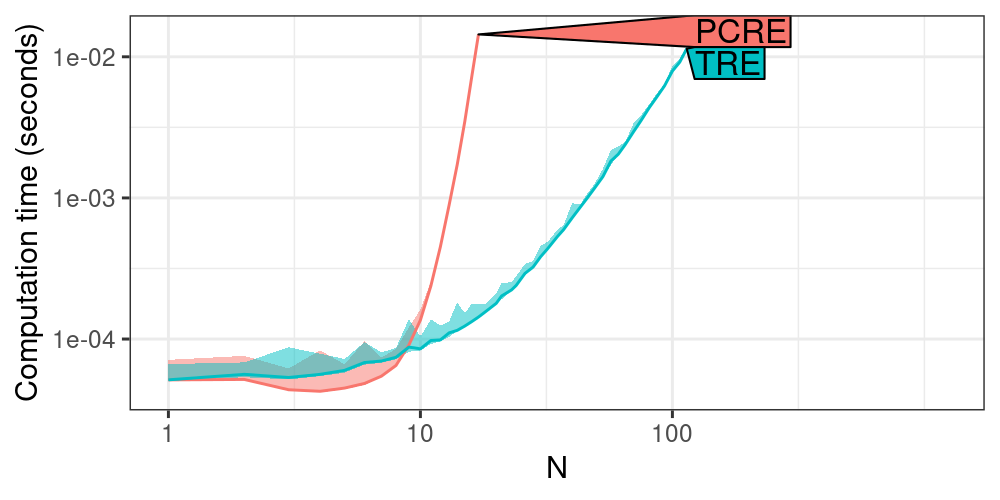
\includegraphics[width=0.9\linewidth]{create_subject_pattern_atime.png}
    \caption{Comparing the computation time for using PCRE and TRE for regex matching with subjects and patterns of size \code{N}.
    Line shows median, and shaded band shows min/max, over 10 timings.}
    \label{fig:plot-atime-PCRE-TRE}
\end{figure}
Note in the code above that the plot method returns a ggplot object, which we modify by adding null facets and a different y scale.
By default, \pkg{atime} measures memory in kilobytes, as well as computation time in seconds.
To simplify the discussion of this first example, we set the \code{unit.col.vec} element in the code above, which ensures that only the computation time is displayed (median line and min/max band over 10 timings).
See Figure~\ref{fig:vector-matrix-length-seconds-kilobytes} for a more complicated example that also shows memory usage.
Figure~\ref{fig:plot-atime-PCRE-TRE} shows the computation time for \code{PCRE} and \code{TRE}, making it easy to see the ranking of these libraries (TRE is faster than PCRE).
\subsection{Asymptotic complexity class estimation}

To estimate the asymptotic complexity class of each expression, we use the code below:
\begin{Schunk}
\begin{Sinput}
> (best.list <- atime::references_best(atime.list))
\end{Sinput}
\begin{Soutput}
references_best list with 61 measurements, best fit complexity:
PCRE (2^N seconds)
TRE (N^3 seconds)
\end{Soutput}
\end{Schunk}
The code above fits an asymptotic reference curve for each of several complexity classes, to each empirical timing curve. 
The complexity classes that are implemented by default include linear $O(N)$, log $O(\log N)$, quadratic $O(N^2)$, exponential $O(2^N)$, etc.
The user can define complexity classes to use, if the defaults are not sufficient. 
An asymptotic reference curve is fit for each complexity class, by aligning it with the empirical timing for the largest $N$ value.  
The output above shows the best fit asymptotic time complexity for each expression, which is defined as the complexity class with the reference curve that is closest to the empirical curve, for the second to largest $N$ value. To visualize the results, we use the code below.
\begin{Schunk}
\begin{Sinput}
> plot(best.list) + ggplot2::facet_grid(. ~ expr.name) +
+   ggplot2::scale_y_log10("Computation time (seconds)")
\end{Sinput}
\end{Schunk}

\begin{figure}[t]
    \centering
    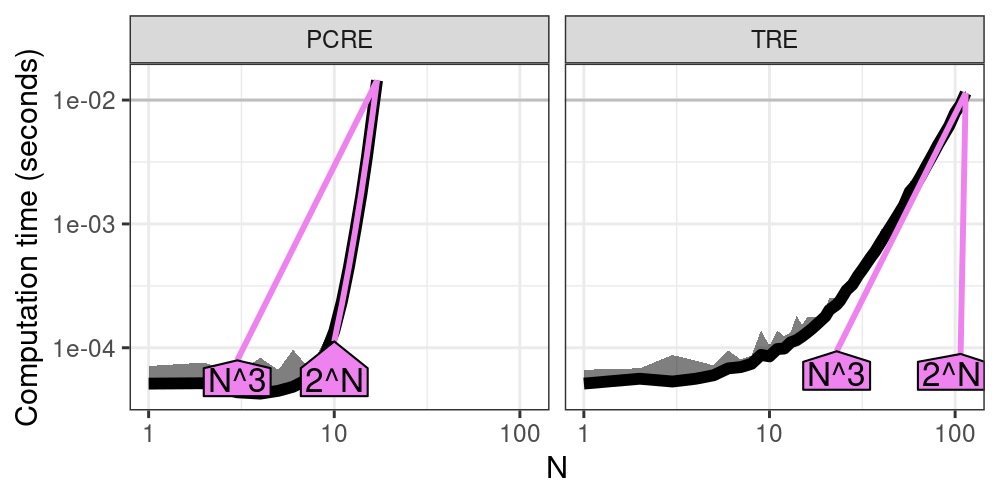
\includegraphics[width=0.9\linewidth]{create_subject_pattern_best.png}
    \caption{Computation time (seconds) as a function of input size $N$ for PCRE and TRE. 
    Empirical timings are shown in black (median line and min/max band over 10 timings), while purple curves show reference asymptotic growth rates: exponential $O(2^N)$ is best fit for PCRE, and cubic $O(N^3)$ is best fit for TRE.}
    \label{fig:plot-best-list-PCRE-TRE}
\end{figure}

Figure~\ref{fig:plot-best-list-PCRE-TRE} shows the timings of each expression as a function of data size $N$ (black), as well as one or two asymptotic reference curves (violet, closest reference curve that is smaller/larger, with text labels that can be interpreted in terms of big O notation).
Since we have chosen $N$ and the time limit appropriately, we are able to observe the following.
For small values of $N$, the timings are dominated by the overhead, resulting in a nearly constant curve (especially for PCRE). 
As $N$ increases, the PCRE curve becomes super-linear, indicating exponential complexity, as shown by the increasing slope in the log-log plot, and the almost perfect alignment between the black empirical curve, and the violet exponential $O(2^N)$ reference curve.
Note that this example is a worst case for the PCRE library, which is actually quite fast for other more typical subjects and patterns.
For \texttt{TRE}, two references are shown: cubic $O(N^3)$ appears to be the best fit, whereas exponential $O(2^N)$ is the closest reference that is slower.
Note that all polynomial references, including cubic $O(N^3)$, appear as linear trends on the log-log plot.
Overall, Figure~\ref{fig:plot-best-list-PCRE-TRE} shows the empirical timings, along with best fit asymptotic reference curves, which indicate that PCRE is exponential time, and TRE is polynomial time, as a function of the size of the subject/pattern $N$.



\subsection{Comparing latency and throughput}

When comparing algorithms in terms of computational resources, we can either compare the time/memory required for a given data size $N$ (latency), or show the data size $N$ possible for a given time/memory budget (throughput).
To compare latency for a given data size, we can simply subset the data table of empirical measurements, as below:
\begin{Schunk}
\begin{Sinput}
> atime.list$measurements[N==15, .(expr.name, seconds=median)]
\end{Sinput}
\begin{Soutput}
   expr.name      seconds
      <char>        <num>
1:      PCRE 0.0034745010
2:       TRE 0.0001235669
\end{Soutput}
\end{Schunk}
The output above shows that TRE is more than ten time faster than PCRE, at the given data size.
To compare throughput, we use the code below.
\begin{Schunk}
\begin{Sinput}
> (pred.list <- predict(best.list))
\end{Sinput}
\begin{Soutput}
atime_prediction object
      unit expr.name unit.value        N
    <char>    <char>      <num>    <num>
1: seconds      PCRE       0.01  16.4573
2: seconds       TRE       0.01 109.7062
\end{Soutput}
\end{Schunk}
The output above shows a table with one row per expression. 
It shows that at the default time limit (0.01 seconds), TRE has a much larger estimated throughput than PCRE (\code{N} column). 
The throughput is estimated using linear interpolation on the log-log plot.
The \code{atime\_prediction} object has a plot method, which can be used to compare throughput, as in the code below.
\begin{Schunk}
\begin{Sinput}
> plot(pred.list) + ggplot2::facet_null() +
+   ggplot2::scale_y_log10("Computation time (seconds)", limits=c(NA, 5e-2))
\end{Sinput}
\end{Schunk}
\begin{figure}[t]
    \centering
    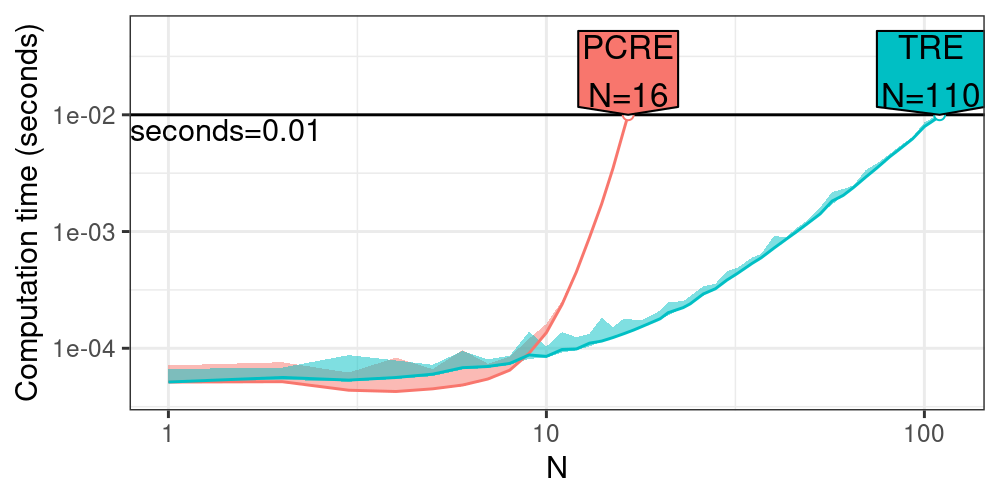
\includegraphics[width=0.9\linewidth]{create_subject_pattern_pred.png}
    \caption{Computation time (seconds) versus data size ($N =$ regex subject/pattern size), highlighting the largest data size $N$ that can be processed within the default time limit of 0.01 seconds. 
    Lines show median, and shaded bands show min/max, over 10 timings.}
    \label{fig:plot-pred-list-PCRE-TRE}
\end{figure}
Figure~\ref{fig:plot-pred-list-PCRE-TRE} shows the throughput, which is the data size N which can be handled in a given amount of time. 
It is clear that the \code{TRE} can handle a larger N for the given time limit.

\section{Analyzing different units as a function of data size}
In this section, we explain how \pkg{atime} can be used to analyze asymptotic properties of other units, in addition to computation time.
We consider the example of creating vectors and matrices of size $N$.
In R, dense matrices are created using \code{matrix}, whereas sparse matrices are created using \code{Matrix}.
The advantage of using a sparse matrix is that when the number of non-zeros is sub-quadratic, then the memory usage should also be sub-quadratic (whereas memory usage with a dense matrix would be quadratic).
In the code below, we use \pkg{atime} to verify these properties, and we also compare with a one-dimensional \code{vector} (linear memory usage). 
Finally, the code below demonstrates usage of the \code{result} argument, which is a function applied to the result of each expression.
Because this function returns a data frame with one row, the column in that data frame (\code{length}) is interpreted as another unit to analyze (in addition to default units, time in \code{seconds} and memory in \code{kilobytes}).
\begin{Schunk}
\begin{Sinput}
> library(Matrix)
> vec.mat.result <- atime::atime(
+   N = 10^seq(1, 7, by=0.25),  
+   vector = numeric(N),
+   matrix = matrix(0, N, N),
+   Matrix = Matrix(0, N, N),
+   result = function(x)data.frame(length = length(x)))
> plot(vec.mat.result)
\end{Sinput}
\end{Schunk}
\begin{figure}[t]
    \centering
    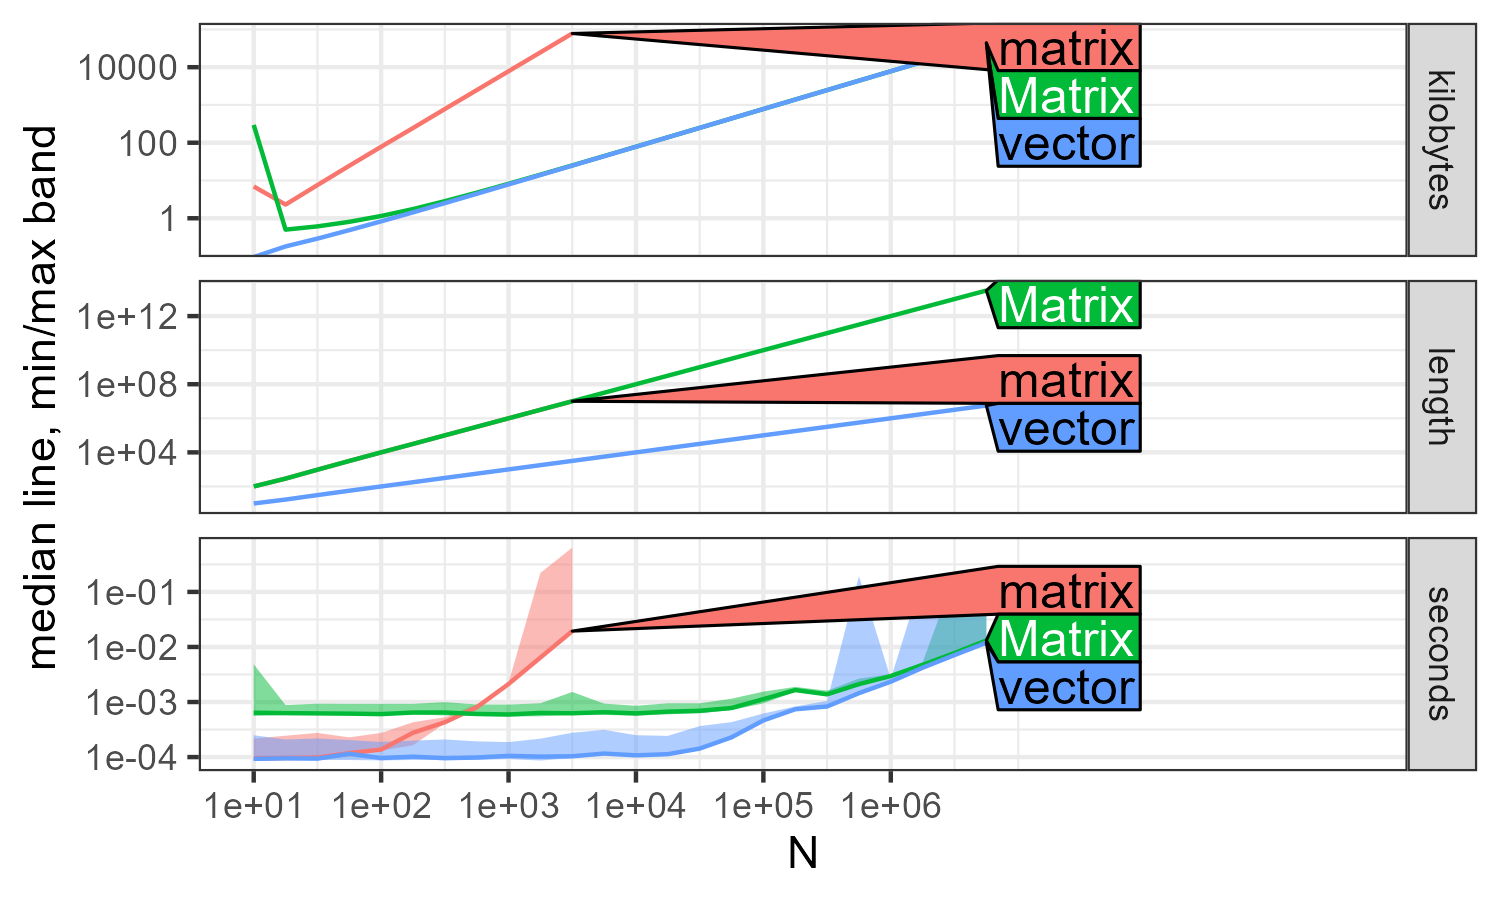
\includegraphics[width=0.9\linewidth]{vec.mat.result.plot.png}
    \caption{Asymptotic comparison of memory usage (kilobytes), object length, and execution time (seconds), for creating a $N$-vector, an $N\times N$ dense matrix, and an $N\times N$ sparse Matrix.
    The seconds panel shows median lines and min/max bands over 10 timings; 
    other panels show a line for the single measurement.}
    \label{fig:vector-matrix-length-seconds-kilobytes}
\end{figure}
The code above creates Figure~\ref{fig:vector-matrix-length-seconds-kilobytes}, in which there are three panels, each representing a different unit of measurement, as a function of data size $N$.
\begin{description}
\item[Kilobytes:] This panel shows memory usage. 
The $N\times N$ sparse \texttt{Matrix} and $N$-\texttt{vector} both exhibit linear $O(N)$ asymptotic memory usage, while $N\times N$ dense \texttt{matrix} requires quadratic $O(N^2)$ memory, as shown by the greater slope in the log-log plot.
\item[Length:] This panel represents the output of the \texttt{length} function. 
Both \texttt{matrix} and \texttt{Matrix} structures have the same quadratic $O(N^2)$ length values, whereas \texttt{vector} has a smaller linear $O(N)$ length asymptotically, as shown by its smaller slope on the log-log plot.
\item[Seconds:] This panel displays execution time. 
For small values of \texttt{N}, \texttt{Matrix} is slower than both \texttt{vector} and \texttt{matrix} due to a small constant overhead. However, as \texttt{N} increases, \texttt{Matrix} and \texttt{vector} converge to the same linear $O(N)$ asymptotic time complexity, much faster than the quadratic $O(N^2)$ time \texttt{matrix} for large \texttt{N}.
\end{description}
As in the previous section, \code{references\_best()} can be used to estimate asymptotic complexity classes, for each of the expressions (\code{matrix}, \code{Matrix}, \code{vector}), and each of the units (kilobytes, length, and seconds). 
Additionally, the \code{predict()} method can be used to estimate the throughput of each expression, for a given limit of seconds, kilobytes, and/or length. 

\section{Performance testing using \pkg{atime}}

The \pkg{atime} package also provides functionality for performance testing R packages that are versioned using git. 
For performance testing an R package, we compute asymptotic time and memory usage for different git versions, and visualize the results to ensure that package code modifications do not result in performance regressions. 
In the context of our paper, a \textit{performance regression} is a significant increase in execution time or memory usage for a particular test case.
In this section, we explain how \pkg{atime} has been used to implement performance testing for \pkg{data.table}, an R package with users that depend on its impressive performance.

The \pkg{atime} package provides functions for prototyping test cases, defining test cases in an R package, and then running the test cases.
The first step of performance testing is typically prototyping, which means experimenting with different test code, package versions, and data sizes, until significant differences in performance can be observed. 
Prototyping is done using \code{atime\_versions()}, which runs a given piece of R code, for several data sizes \code{N}, and for several package versions (defined using git SHA1 hashes).
After prototyping, the arguments used with \code{atime\_versions()} can be re-used with \code{atime\_test()}, which is used to define test cases in an R package.
Finally, \code{atime\_pkg()} can be used to run all test cases in an R package, or \verb|atime_pkg_test_info()| can be used to extract test meta-data, and run one test at a time.

\subsection{Prototyping performance tests using \code{atime\_versions()}}

The first step of performance testing is typically using \code{atime\_versions()} for prototyping.
Some arguments of \code{atime\_versions()} are the same as \code{atime()}: \code{N} is a sequence of data sizes, and \code{setup} is an expression to create data for use in the test. 
The different package versions are specified as named arguments (\code{Fast} and \code{Slow} in the code below) whose values should be SHA1 hashes of the desired git versions.
Additionally \code{pkg.path} is the path to a local clone of a git repository containing the R package, and \code{expr} is an expression to time for each different package version.
Note that this expression must contain a double or triple colon reference to the package name, such as \code{data.table:::setDT} in the code below.
Testing the different versions is implemented by installing different versions of the package, to the same R package library.
The different package versions have different names, so can be loaded and run in the same R session.
The names of the different R packages are created by appending the SHA1 hash to the package name, for example \code{data.table.c4a2085e35689a108d67dacb2f8261e4964d7e12}.
The \code{pkg.edit.fun} argument is a function to edit the package, so that it can be installed and loaded using the versioned package name.
A default \code{pkg.edit.fun} is provided that works with most R packages (including packages that use the \pkg{Rcpp} interface of \citet{Rcpp}), but \pkg{data.table} has some special configuration that required creating a custom function, \code{edit.data.table} (see GitHub repository for details). 
We consider the example usage in the code below.
\begin{Schunk}
\begin{Sinput}
atime::atime_versions(
  pkg.path = "~/data.table",
  pkg.edit.fun = edit.data.table, 
  setup = {
    set.seed(1L)
    dt <- data.table(a = sample.int(N))
    setindexv(dt, "a")
  },
  expr = data.table:::shallow(dt),
  Slow = "b1b1832b0d2d4032b46477d9fe6efb15006664f4", 
  Fast = "9d3b9202fddb980345025a4f6ac451ed26a423be")
\end{Sinput}
\end{Schunk}
The code above runs a performance test on two different versions of the \pkg{data.table} package (Fast and Slow), involving computing an index for tables with varying numbers of rows $N$.
It is expected that this operation should be constant $O(1)$ time, independent of the number of columns $N$.
When we use the \code{plot} method (Figure~\ref{fig:plot-perf-test-fast-slow}, left), we see that the Slow version time is increasing with $N$, whereas the Fast version time is constant.
Results like this, where significant differences can be observed between package versions, indicate that the \verb|atime_versions()| code is a good candidate for a performance test. 
To conclude this section, \pkg{atime} provides \code{atime\_versions()} function, which can be used to compare the asymptotic performance of two git versions of an R package.

\begin{figure}[t]
    \centering
    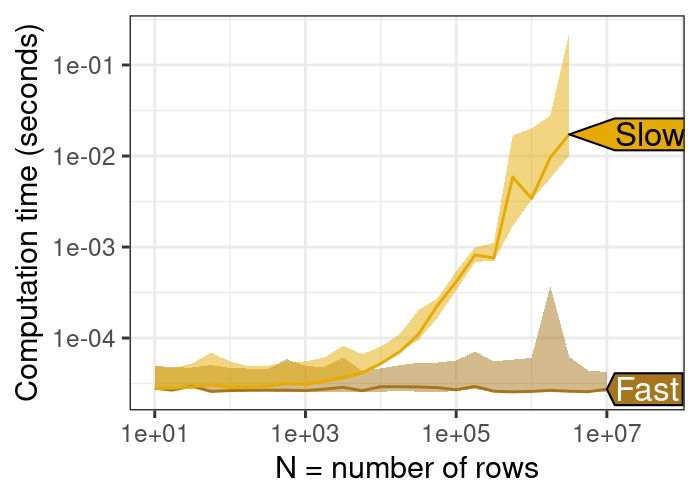
\includegraphics[height=1.8in]{data.table-atime_versions.png}
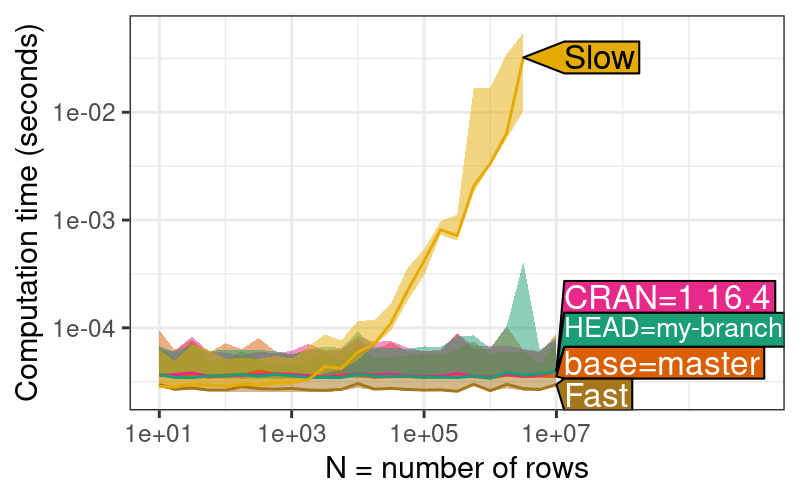
\includegraphics[height=1.8in]{data.table-atime_test.png}
     \caption{\textbf{Left:} \code{plot} method for \code{atime\_versions()} shows asymptotic time taken for \code{shallow()}, which performs a shallow copy of a data table with $N$ rows, an operation which is expected to be constant time (as in Fast version, but not Slow version).
     \textbf{Right:} same test case run in the context of a Pull Request on GitHub, resulting in three additional versions (CRAN, HEAD, base).
     It is clear that all versions other than Slow are about the same speed as Fast, which indicates that HEAD is OK to merge into base.}
    \label{fig:plot-perf-test-fast-slow}
\end{figure}


\subsection{Defining performance tests in an R package}
After having used \verb|atime_versions()| to prototype a performance test, the next step is to move the test code into the R package. 
We propose defining performance test cases in the object named \code{test.list} defined in the \code{pkg/.ci/atime/tests.R} file in a git repository \code{pkg} containing an R package.
Each element of the list should have an informative name, that will be used to display the results.
Each value should be a list of named arguments to pass to \verb|atime_versions()|, such as \code{setup}, \code{expr}, \code{Fast}, and  \code{Slow}.
Each test case is typically created based on a historical regression or performance improvement. 
For example, the R code below defines the test case involving \code{shallow}, as discussed in the previous section.
\begin{Schunk}
\begin{Sinput}
test.list <- atime::atime_test_list(
  N = as.integer(10^seq(1, 7, by=0.25)),
  pkg.edit.fun = edit.data.table,
  "shallow speed improved in #4440" = atime::atime_test(
    setup = {
      set.seed(1L)
      dt <- data.table(a = sample.int(N))
      setindexv(dt, "a")
    },
    expr = data.table:::shallow(dt),
    Slow = "b1b1832b0d2d4032b46477d9fe6efb15006664f4", 
    Fast = "9d3b9202fddb980345025a4f6ac451ed26a423be"
  )
)
\end{Sinput}
\end{Schunk}
The code above uses the helper functions \verb|atime_test_list()| and \verb|atime_test()| to define the test case.
Both functions are wrappers around \code{list()}, with non-standard evaluation for special arguments like \code{setup} and \code{expr} (un-evaluated expressions to pass to \verb|atime_versions|). 
The arguments \code{N} and \code{pkg.edit.fun} are special names that are recognized by \verb|atime_test_list|, and shared across all of the test cases in the list (only one test case shown above; see \pkg{data.table} repository for more).
In addition to the code above, it is recommended to add names and/or comments that explain the origin of the test case.
For example, the test case name \code{"shallow speed improved in \#4440"} references the PR number which resulted in the performance improvement.
Also, for each SHA1 hash, we recommend a comment such as the following, which was used to document the origin of the Slow commit:
\code{Parent of the first commit (\url{https://github.com/Rdatatable/data.table/commit/0f0e7127b880df8459b0ed064dc841acd22f5b73}) in the PR (\url{https://github.com/Rdatatable/data.table/pull/4440/commits}) that improves speed}.
Such comments are useful because they can be used to double check the validity of the SHA1 commit IDs.
In this example, on the PR4440 web page, it can be seen that 0f0e712 is the first commit, and on that commit page, it can be seen that b1b1832 is indeed its parent (which is a good choice for a historical Slow reference because it occurred before the PR that introduced the performance improvement).

\subsection{Running performance tests locally and on GitHub Actions}


\paragraph{Running performance tests locally.}
After having defined test cases as above, all the test cases in the package can be run locally by using \verb|atime_pkg("path/to/pkg")|.
It runs \verb|atime_versions()| using the arguments provided in each test case, and then saves the results (RDS file), along with summary PNG figure files, to the directory \code{pkg/.ci/atime}.
Alternatively, to run and visualize the results for a single test case, code as below can be used.
\begin{Schunk}
\begin{Sinput}
pkg.info <- atime::atime_pkg_test_info("~/R/data.table")
one.call <- pkg.info$test.call[["shallow regression fixed in #4440"]] 
one.result <- eval(one.call) 
plot(one.result)
\end{Sinput}    
\end{Schunk}
The \verb|atime_pkg_test_info()| function returns a list of information about the performance test cases, without actually running them yet.
The \verb|pkg.info$test.call| object is a list of un-evaluated expressions, each of which calls \verb|atime_versions()| for a given test case.
The code \code{eval(one.call)} runs one performance test, and the plot method can be used to visualize the results (Figure~\ref{fig:plot-perf-test-fast-slow}, right).
Running the test case locally adds three versions (Table~\ref{tab:version-labels}): HEAD (current git version in local clone), base (\verb|GITHUB_BASE_REF| or master), and CRAN (current release).
The performance of these versions can be compared to the historical commits (Fast and Slow), to evaluate the performance of the current code.

\paragraph{Running performance tests on GitHub Actions.}

GitHub Actions is a continuous integration service that can run arbitrary code after every push to a git repository.
A GitHub Action was created to facilitate performance testing of the changes that are introduced in a Pull Request (PR). 
The primary motivation behind this was to help ensure that \pkg{data.table} maintains its code efficiency as PRs are merged.
The Github Action for performance testing can be enabled by creating a YAML file in \code{pkg/.github/workflows} (see atime web page for details).
The GitHub Action first runs \verb|atime_pkg()| after each push to a branch involved in a PR.
The GitHub Action then creates a comment in the PR, with the summary figure that shows the result from the most recent performance test.
The comment gets updated after each push, to avoid cluttering the PR.
The plot shows a column for each test case, with time and memory trends across different \code{data.table} versions (Table~\ref{tab:version-labels}).
In addition, the comment contains a link to download all the \code{atime}-generated result files (figure PNG files and RDS).

Several versions are provided automatically by atime, based on the context of the PR (base, HEAD, merge-base, CRAN).
Other versions can be provided by the user based on what is relevant for each test case (Before, Regression, Fixed, Fast, Slow).
For test cases that involve a regression, we recommend the version names Before, Regression, and Fixed, to indicate versions relative to the regression (Before and Fixed should be more efficient than Regression).
For test cases that involve a performance improvement (or no known regression), we recommend using the version names Fast and Slow.
\begin{table}[t]
        \centering
            \caption{\label{tab:version-labels}Version names recognized by atime performance testing. }
        \begin{tabular}    
        {|m{2.2cm}|m{1.5cm}|m{9cm}|}
  \hline
      \textbf{Version name} & \textbf{Defined?} & \textbf{Version description} \\
  \hline
  Fast & user & An efficient commit \\
  \hline
  Slow & user & An inefficient commit\\
  \hline
  Before & user & An efficient commit before a performance regression  \\
  \hline
  Regression & user & An inefficient commit affected by a performance regression \\
  \hline  
   Fixed & user & An efficient commit after  fixing a performance regression \\
  \hline  
  CRAN & local & Latest version on CRAN  \\
  \hline
  HEAD & local &  Most recent commit in current branch \\
  \hline
  base & GitHub & Target branch of PR (typically main or master), if current branch involved in a PR \\
  \hline
  merge-base & GitHub & The common ancestor between base and HEAD \\
  \hline
    \end{tabular}
\end{table}





\section{Comparisons between \pkg{atime} and other software}

\subsection{Comparing \pkg{atime} and  \pkg{touchstone} for performance testing}

The most similar R package to \pkg{atime} is \pkg{touchstone}, which implements similar ideas for performance testing, but without asymptotic measurement (for variable data size N). 


Both \pkg{touchstone} and \pkg{atime} use relative performance testing, meaning that each test case is run using different versions of the R package.
Touchstone allows specifying two branches, corresponding to the HEAD of a PR, and its base branch.
In addition to those branches, \pkg{atime} supports other branches which are important in the context of a PR (merge-base and CRAN), as well as user-defined commits that represent historical Fast/Slow versions.

\verb|touchstone::branch_install()| installs each branch to a separate library, and uses \pkg{callr} to run each branch in a separate R process.
In contrast, \verb|atime::atime_versions()| installs each package version to the same library (using a different package name for each version).
Therefore, \pkg{atime} allows the different R package versions to be loaded into the same R session, for more direct comparison (reduced noise).

\section{Comparative benchmarking using \code{atime::atime()} and \code{bench::press()}}


In terms comparative benchmarking functionality, the function most similar to \code{atime::atime()} is \code{bench::press()}, which allows the user to specify several parameters to vary (not only data size \code{N}).
The main advantage of \pkg{atime} is that it provides certain convenient features for benchmarking code that scales with data size, $N$. 

\paragraph{Simple example with small data size $N$, for which bench and atime work equally well.}
The \pkg{bench} package can be used for asymptotic benchmarking, as long as the max data size $N$ is chosen to yield a reasonable computation time for all expressions.
For example, \pkg{bench} can be used to do a small-scale asymptotic comparison of PCRE and TRE, via the code below. 
\begin{Schunk}
\begin{Sinput}
bench::press(
  N = 1:20,
  perl = c(TRUE, FALSE),
  with(create_subject_pattern(N), bench::mark(
    iterations = 10,
    regexpr(pattern, subject, perl = perl))))
\end{Sinput}
\end{Schunk}
The code above is an attempt to replicate Figure~\ref{fig:plot-atime-PCRE-TRE}, but with smaller data sizes (max=20 instead of 100, which would be too slow to compute using PCRE).
In the code above, we use the \texttt{bench::press()} function to perform benchmarking across multiple parameter combinations (\texttt{N} and \texttt{perl}).
For each combination, it calls the \texttt{create\_subject\_pattern} function with the current \texttt{N} to generate a \texttt{subject} and \texttt{pattern}, and subsequently measures the performance of the \texttt{regexpr} function using \texttt{bench::mark()}. The \texttt{regexpr} function performs regular expression matching with the generated \texttt{pattern} on the \texttt{subject}, using the current value of \texttt{perl} to toggle Perl-compatible regex. 
The benchmarking process is repeated \code{iterations = 10} times for each parameter combination.
% Figure~\ref{fig}
Below we show the analogous \pkg{atime} code. 
\begin{Schunk}
\begin{Sinput}
atime::atime(
  N = 1:20,
  setup = N.data <- create_subject_pattern(N),
  expr.list = atime::atime_grid(
    list(perl = c(TRUE, FALSE)),
    regexpr = regexpr(N.data$pattern, N.data$subject, perl = perl)))
\end{Sinput}
\end{Schunk}
The code above uses the \texttt{expr.list} argument, which is a list of expressions to be benchmarked, constructed using \texttt{atime::atime\_grid}, which defines a grid of parameter combinations (similar to \code{bench::press}). 
In this case, the grid includes one parameter, \texttt{perl}, with values \code{TRUE} or \code{FALSE}. 
Overall, we see from this example that the \pkg{atime} and \pkg{bench} code is very similar, for the case where the max data size $N$ is small enough to be computable by all expressions.



\paragraph{More complex example showing the advantage of atime.}
An example that is more difficult to handle using \verb|bench::press| would be the analysis presented in Figure~\ref{fig:vector-matrix-length-seconds-kilobytes}, which shows an extra unit (length, in addition to seconds and kilobytes), and involves very different time/memory scales (dense \texttt{matrix} is orders of magnitude less efficient than sparse \texttt{Matrix}).
That analysis requires two useful features that are provided by \code{atime}. 
\begin{itemize}
\item To measure quantities other than seconds and kilobytes as a function of N (such as length in Figure~\ref{fig:vector-matrix-length-seconds-kilobytes}), then a custom for loop is required with \verb|bench::press()|.
\item If an expression takes longer than the time limit (default 0.01 seconds), then custom code is required for \verb|bench::press()| to not be run for any larger N values. 
And in the case of Figure~\ref{fig:vector-matrix-length-seconds-kilobytes} it is also important to avoid running the large N values, in order to avoid running out of memory.
\end{itemize}
The code below can be used to achieve these two features using \verb|bench::press()|, but it is complicated relative to the corresponding \verb|atime| code that was used to create Figure~\ref{fig:vector-matrix-length-seconds-kilobytes} (see previous section above).

\begin{Schunk}
    \begin{Sinput}
seconds.limit <- 0.01
done.vec <- NULL
measure.vars <- c("seconds","kilobytes","length")
press_result <- bench::press(N = N_seq, {
  exprs <- function(...)as.list(match.call()[-1])
  elist <- exprs(
    vector=numeric(N),
    matrix=matrix(0, N, N),
    Matrix=Matrix(0, N, N))
  elist[names(done.vec)] <- NA #Don't run exprs which already exceeded limit.
  mark.args <- c(elist, list(iterations=10, check=FALSE))
  mark.result <- do.call(bench::mark, mark.args)
  desc.vec <- attr(mark.result$expression, "description")
  mark.result$description <- desc.vec
  mark.result$seconds <- as.numeric(mark.result$median)
  mark.result$kilobytes <- as.numeric(mark.result$mem_alloc/1024)
  mark.result$length <- NA
  for(desc.i in seq_along(desc.vec)){
    description <- desc.vec[[desc.i]]
    result <- eval(elist[[description]])
    mark.result$length[desc.i] <- length(result)
  }
  mark.result[desc.vec %in% names(done.vec), measure.vars] <- NA
  over.limit <- mark.result$seconds > seconds.limit
  over.desc <- desc.vec[is.finite(mark.result$seconds) & over.limit]
  done.vec[over.desc] <<- TRUE
  mark.result
})
    \end{Sinput}
\end{Schunk}
The code above uses entries of \verb|done.vec| to keep track of which expressions have already gone over the time limit.
It also uses a for loop to evaluate each expression and save the length of the result to analyze as a function of N.
Overall the code is substantially more complex than the corresponding \pkg{atime} code, because it has to re-implement two features that \pkg{atime} provides.

To conclude this section, we have discussed the use of \pkg{bench} and \pkg{atime} packages for comparative benchmarking in R. 
Both methods can be used for comparative benchmarking across different parameter configurations. 
However, \code{atime::atime()} provides two key features which are not present in \verb|bench::press()|: measurement of arbitrary units (other than time and memory), and stopping evaluation for expressions that go over a time limit.

\section{Discussion and conclusions}

In this paper, we presented the \pkg{atime} package for comparative benchmarking R code, and performance testing R packages. 
The \pkg{atime} package enables users to compute and visualize asymptotic timings, including comparing empirical timings with theoretical references, and estimating throughput.
Several examples illustrated how \pkg{atime} can be applied for comparative benchmarking of different R functions that perform similar computations (but with different performance characteristics).
Using \pkg{data.table} as an example, we explained how \pkg{atime} can be used for performance testing of R packages across multiple git versions. 

Additionally, we compared \pkg{atime}'s syntax and functionality with other tools used for performance testing and benchmarking. 
Compared to other benchmarking tools (which support only a single data size), the unique feature of \pkg{atime} is support for sequences of data sizes. 
We showed that it is technically possible to use \code{bench::press()} for asymptotic analysis across a sequence of small data sizes, but \pkg{atime} is preferable because it supports convenience features such as stopping if a timing exceeds a time limit.
Another similar package is \pkg{touchstone}, which provides a GitHub Action for performance testing based on comparing HEAD/base versions, but does not support asymptotic analysis (varying data sizes).

Finally, we note that \pkg{atime} is currently being used for continuous performance testing of \pkg{data.table}, with 16 test cases currently implemented, and running for every pull request on GitHub.
The \pkg{atime} methodology has also been used to uncover and fix asymptotic performance issues in base R.
For example, asymptotic analysis of \code{write.csv} revealed that it was quadratic $O(N^2)$ in the number of columns $N$, whereas the expected complexity was linear $O(N)$.
Sebastian Meyer realized this issue was related to another issue with replacing columns via \verb|[.data.frame|, which was observed to be super-linear, but expected to be linear.
The fix for these two issues appeared in 2023 with R version 4.3.0.
Other examples include \code{substring} which was expected to be linear $O(N)$ time in the number of outputs $N$, and \code{gregexpr} which was expected to be linear $O(N)$ time in the number of characters $N$ in the subject. 
Our asymptotic analysis revealed that both operations were quadratic $O(N^2)$ time, and Tomas Kalibera merged the proposed fixes into R version 3.6.0 (2019).
Overall, we have shown how \pkg{atime} simplifies such asymptotic analysis, and we expect that it will be a useful tool for future analyses of other R functions.



\newpage
\bibliography{DorisAmoakohene}